\chapter{Tests \& Results}

\section{Tests}
This section presents highlights from the testing suite of the pipelined MIPS processor with speculative execution. Branch prediction, data forwarding (including load-store forwarding), and pipeline flushing is demonstrated executing successfully.

\subsection{System integration test}

The provided system integration test from exercise 1 (see Figure \ref{fig:toplevel_sim}),
which tests basic load, store, jump and arithmetic, was successfully run on the pipelined architecture.
The testbench has been extended to be more thorough, checking that the data from store
instructions following a branch taken doesn't end up in memory.

\subsection{Store after load operand forwarding}

The presented architecture has been extended to support operand forwarding from the write-back pipeline stage to the memory stage.
This allows for load instructions to be followed by store instructions without having to insert pipeline bubbles.

\begin{figure}[H]
  \begin{code}
    lui $3, 2
    srl $3, $3, 16   # Load 2 to $3
    lw $3, 1($0)     # Loads 1 from memory
    sw $3, 3($0)     # Should store 1, not 2 to address 3
  \end{code}
  \caption{Assembly to test store after load operand forwarding}
  \label{fig:test-store-after-load}
\end{figure}

Expected behavior:
\begin{itemize}
  \item
    The sw instruction should store the newly loaded value from the lw instruction, in effect acting like a memory move instruction.
  \item
    Bubbles should not be inserted into the pipeline.
\end{itemize}

\subsubsection*{simulation results}

\begin{figure}[H]
  \begin{center}
    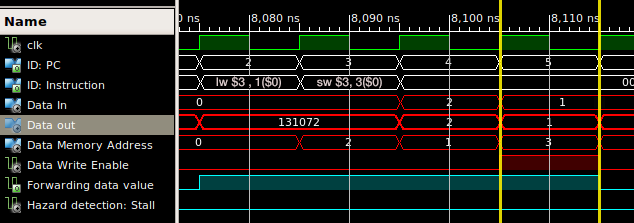
\includegraphics[width=\textwidth]{assets/lw-sw-forwarding.png}
  \end{center}
  \caption{
    Store after load simulation}
  \label{fig:simulate_lw_sw}
\end{figure}

Instructions 2 and 3 (lw and sw) are in the wb and mem stages, respectively, in the yellow area of simulation image \ref{fig:simulate_lw_sw}.
Notice that 'data write enable' is asserted by the sw instruction, and 'forwarding data value' by the forwarding unit.
The value on the 'data out' line equals the value on the 'data in' line. Forwarding has completed successfully.

The hazard detection stall signal was never asserted, i.e. no bubbles were inserted.

\subsection{Branch prediction}

The test case in figure \ref{fig:test-branch-prediction} tests both the hazard detection and branch prediction capabilities of the processor.

\begin{figure}[H]
  \begin{code}
    lw $1, 0($0)
    lw $2, 1($0)      # Should stall after this instruction (data hazard).
    beq $2, $0, 3     # Should predict (Control hazard).
    sw $2, 2($0)
    sub $2, $2, $1    # Introduce data hazard for beq
    j 2               # Jump to loop condition
    beq $0, $0, -1    # Loop forever
  \end{code}
  \caption{Assembly to test branch prediction} \label{fig:test-branch-prediction}
\end{figure}

Expected behavior:
\begin{itemize}
  \item
    The pipeline stalling on instruction 2. Branch after load requires one stall cycle to actually be able to correct for wrongly taken branches.
  \item
    The processor predicting whether instruction 2 should branch or not.
    Operands are available neither the first time (load not having completed yet), or after the end-of-loop jump (the sub instruction not having completed yet).
    As this architecture doesn't support operand forwarding to the branch predictor, it will have to guess.
\end{itemize}

\subsubsection*{simulation results}

\begin{figure}[H]
  \begin{center}
    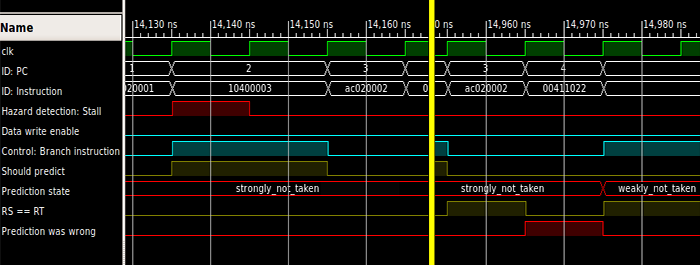
\includegraphics[width=\textwidth]{assets/branch-prediction.png}
  \end{center}
  \caption{Branch prediction simulation}
  \label{fig:simulate_branch_prediction}
\end{figure}

Consider the left part of simulation \ref{fig:simulate_branch_prediction}.
The data dependency between instruction 1 and 2 is detected, resulting in a one cycle stall as instruction 1 reaches the decode stage.
The 'Control: branch' signal is also asserted, sampling a suggestion from the branch predictor.
The two bit predictor has to be used, as operands aren't available yet. It suggests not taking the branch.
This turns out being the correct choice, requiring no corrective action.

In the right part of simulation \ref{fig:simulate_branch_prediction}, one can barely see the end of the last branch instruction of the loop.
The branch predictor has to speculate yet again, and uses the choice that has worked for the last n-1 iterations: branch not taken.
Sadly, not all branches can be taken and the choice ends up wrong.
Two cycles later the error is noticed, and the 'prediction was wrong' signal is asserted.
The branch predictor takes this suggestion to heart, and decides to switch state to 'weakly not taken'.

\subsection{Pipeline flushing}

The test case in figure \ref{fig:test-pipeline-flushing} tests that speculatively executed instructions are correctly flushed from the pipeline.

\begin{figure}[H]
  \begin{code}
    lw $2, 2($0)    # Loads 2 into $2
    lw $1, 1($0)    # Loads 0 into $1
    beq $1, $0, 2   # Branch speculatively not taken
    sw $2, 4($0)    # Speculatively executed, to be flushed
    j 6             # Speculatively executed, to be flushed
    sw $1, 5($0)    # Should actually be executed
  \end{code}
  \caption{Assembly to test pipeline flushing}
  \label{fig:test-pipeline-flushing}
\end{figure}

Expected behavior:
\begin{itemize}
  \item
    Instructions 3 and 4 should be speculatively executed, and flushed.
  \item
    Memory address 5 should have the value 2, address 4 should have the value 0.
\end{itemize}

\subsubsection*{simulation results}

\begin{figure}[H]
  \begin{center}
    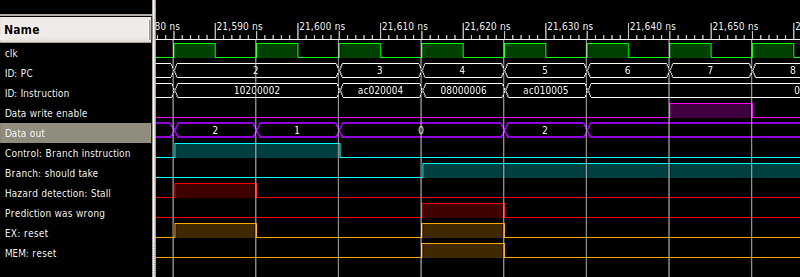
\includegraphics[width=\textwidth]{assets/pipeline-flushage.png}
  \end{center}
  \caption{Simulation of pipeline flushing}
  \label{fig:simulate_pipeline_flushing}
\end{figure}

After stalling for one cycle on instruction 2 (beq) due to the data dependency on the lw preceding it, the branch predictor guesses not taken, and speculative execution of instructions 3 and 4 begins.
The prediction is confirmed wrong as instruction 4 enters the ID stage, and pipeline stages EX and MEM are flushed by asserting their respective reset signals.
Note that instruction 3 (sw) correctly puts '2' on the data out line, but doesn't asserts the data write signal, as it has been flushed.

Further down, we see that instruction 5 successfully stores '0', by asserting the data write signal.

\section{Component Tests}

All tests are written in VHDL and simulated in ISim.
Each component has been tested and verified with a testbench designed to confirm normal operation and detect edge-cases in the behavior.
The results of the tests, as well as their purpose, are shown in table \ref{table:vhdl_component_tests}.

\begin{table}[h]
    \begin{tabular}{|l|p{9cm}|l|}
    \hline
    \textbf{Unit under test} & \textbf{Test purpose}               & \textbf{Test status} \\ \hline
    PC                & Does the program counter increment normally? & \checkmark Passed \\ \cline{2-2}
                      & Can the program counter be paused? & \\ \cline{2-2}
                      & Is the correct order of overrides respected (branch predict, jump, branch correct)? & \\ \hline
    Forwarding unit   & Can data be forwarded from MEM stage to EX stage? & \checkmark Passed \\ \cline{2-2}
                      & Can data be forwarded from WB stage to EX stage? & \\ \cline{2-2}
                      & Can data be forwarded from WB stage to MEM stage? & \\ \cline{2-2}
                      & Is \$r0? ignored & \\ \cline{2-2}
                      & Will it incorrectly forward when control\_reg\_write is not enabled? & \\ \hline
    Two bit predictor & Confirm that the predictor defaults to 'not taken'. & \checkmark Passed \\ \cline{2-2}
                      & Check that two missed predictions are required before prediction switches. & \\\cline{2-2}
                      & Confirm that it properly resets to 'not taken'. & \\ \hline
    Hazard detection  & Confirm that the pipeline doesn't stall when an r-type instruction follows a load, but there's no overlap in registers & \checkmark Passed \\ \cline{2-2}
                      & Check that the pipeline stalls when a memory read precedes a dependent r-type or branch instruction. & \\\cline{2-2}
                      & Check that the pipeline doesn't stall when a data-dependent store instruction follows a load instruction. & \\ \hline
    Control unit      & Confirm that appropriate control signals are output for all supported instructions. & \checkmark Passed \\ \cline{2-2}
                      & Confirm that all outputs are zero when processor is not enabled. & \\ \hline
    \end{tabular}
    \caption{VHDL component tests}
    \label{table:vhdl_component_tests}
\end{table}

\section{Results}

\subsection{Performance}
\todo{Throughput and clock frequency analysis compared to the multi-cycle design. Critical path and such}
\todo{Clock cycle comparison on system integration test, and the loop testbench}
\todo{Take inspiration from the previous report. Same tables and such}

\subsection{Power efficiency}

The MIPS processor makes use of the whole pipeline as much as possible.
By always filling up the pipeline and overlaying instructions, it makes sure as few cycles as possible are wasted.
This makes it so that the total execution time of programs is significantly reduced, which in turn reduces the total static power consumption by allowing earlier return to lower power modes.
The usage of block ram and other dedicated FPGA resources provides additional power savings.
Also, a high maximum clock frequency (62.38 MHz) ensures that each part of the pipeline is executed quickly.

A post-place-and-route power data from Xilinx ISE gives a rough idea of what actual power consumption might look like, see table \ref{tab:power_consumption}.
Even though these values are inaccurate, they can still be used in estimates.

A huge percentage of total power consumption comes from quiescent power draw (simply keeping the FPGA active).
As the processor itself uses very little power, further improvements would be to implement sleeping for inactive states, as well as switching to a more power efficient FPGA.
This would greatly reduce the power consumption of the processor.

\begin{table}[h]
    \centering
    \begin{tabular}{|l|l|}
        \hline
        \textbf{On-Chip} & \textbf{Power (mW)} \\ \hline
        Clocks           & 1.74                \\ \hline
        Logic            & 0.27                \\ \hline
        Signals          & 0.57                \\ \hline
        IOs              & 0.04                \\ \hline
        16k BlockRAM     & 1.43                \\ \hline
        Quiescent        & 24.00               \\ \hline
        \textbf{Total}   & 28.06               \\ \hline
    \end{tabular}
    \caption{Power estimates from Xilinx ISE}
    \label{tab:power_consumption}
\end{table}
